\usetikzlibrary{shapes.multipart,positioning}
\newcommand{\fourdigits}[1]{%
\ifnum #1<10 0%
\fi%
\ifnum #1<100 0%
\fi%
\ifnum #1<1000 0%
\fi% 
\number #1
}
\tikzset{bucket/.style={draw,rectangle split,rectangle split
horizontal,rectangle split parts=#1,text width=.5cm,anchor=west},
mybox/.style={rectangle,draw,minimum width=1.5cm,minimum height=0.5cm}}
\newcommand{\mybucketfour}[7][]{
\node[bucket=4,#1] (#2){#4
\nodepart{two}
#5
\nodepart{three}
#6
\nodepart{four}
#7
};
\node[draw,above left=0pt of #2.north west,anchor=south west,fill=gray!30,
text width=.5cm,yshift=-\pgflinewidth]{\textbf{#3}};
}
\newcommand{\Connect}[3][-latex]{\draw[#1] (#2) to[out=0,in=180] (#3);
}

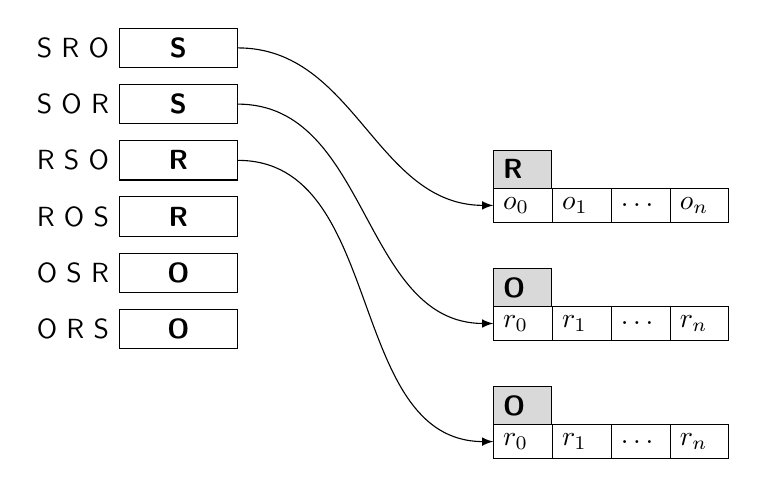
\begin{tikzpicture}[font=\sffamily,node distance=1.5cm]
    % directory
    \begin{scope}[xshift=-4cm,yshift=2cm]   
    \node[mybox,label=left:{S R O}, alias=directory-a] (box-a) {\textbf{S}};
    \node[mybox,below=0.2cm of box-a,label=left:{S O R}, alias=directory-b] (box-b) {\textbf{S}};
    \node[mybox,below=0.2cm of box-b,label=left:{R S O}, alias=directory-c] (box-c) {\textbf{R}};
    \node[mybox,below=0.2cm of box-c,label=left:{R O S}, alias=directory-d] (box-d) {\textbf{R}};
    \node[mybox,below=0.2cm of box-d,label=left:{O S R}, alias=directory-e] (box-e) {\textbf{O}};
    \node[mybox,below=0.2cm of box-e,label=left:{O R S}, alias=directory-f] (box-f) {\textbf{O}};
    \end{scope}
    % buckets
    \mybucketfour{RO}{R}{$o_0$}{$o_1$}{$\ldots$}{$o_n$}
    \mybucketfour[below=of RO.west,anchor=west]{OR}{O}{$r_0$}{$r_1$}{$\ldots$}{$r_n$}
    \mybucketfour[below=of OR.west,anchor=west]{SO}{O}{$r_0$}{$r_1$}{$\ldots$}{$r_n$}
    % links
    \Connect{directory-a}{RO}
    \Connect{directory-b}{OR}
    \Connect{directory-c}{SO}
    %\Connect{directory-0011}{D}
    %\Connect{directory-0100}{A2}
    %\Connect{directory-0101}{B}
\end{tikzpicture}
